\chapter{TINJAUAN PUSTAKA}
\label{chap:tinjauanpustaka}

% Ubah bagian-bagian berikut dengan isi dari tinjauan pustaka

Demi mendukung penelitian ini, tinjauan pustaka membahas beberapa aspek penting
ter-kait pengembangan platform tiket konser berbasis blockchain.

\section{Blockchain dan Teknologi Desentralisasi}
\label{sec:blockchainddanteknologidesentralisasi}
Teknologi blockchain pertama kali diperkenalkan oleh Satoshi Nakamoto dalam
maka-lah berjudul `Bitcoin: A Peer-to-Peer Electronic Cash System' pada tahun
2008 \parencite{nakamoto2008bitcoin}. Pada makalah tersebut, Nakamoto
mengusulkan sistem peer-to-peer untuk menyelesaikan masalah double-spending
dalam sistem pembayaran elektronik yang terdesentralisasi, tanpa memerlukan
pihak ketiga sebagai verifikator. Sistem ini memungkinkan jaringan
memverifikasi transaksi yang diajukan dengan memeriksa riwayat transaksi
sebelumnya. Transaksi yang telah diverifikasi dalam suatu periode waktu
diorganisasi ke dalam struktur Merkle Tree untuk membentuk blok baru. Dalam
transaksi yang melibatkan pengirim yang sama, hanya transaksi pertama yang akan
diterima, guna mencegah terjadinya double-spending. Setiap blok memiliki hash
dari blok sebelumnya, membentuk rantai yang saling terhubung. Setelah blok baru
dihasilkan, blok tersebut akan disiarkan ke seluruh node di jaringan untuk
diverifikasi. Jika lolos verifikasi, blok tersebut ditambahkan ke rantai blok
yang ada.

\begin{figure} [H] \centering
  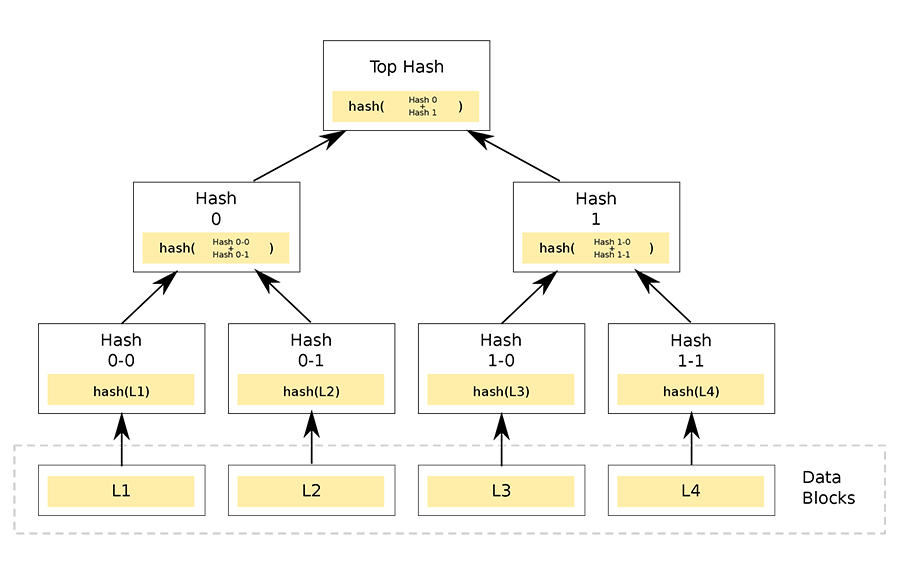
\includegraphics[scale=0.45]{gambar/bab2/merkle-hash-tree.png}
  \caption{Merkle Tree Methodology \parencite{MerkleTree}}
  \label{fig:MerkleTree}
\end{figure}

Node di dalam jaringan selalu mengikuti rantai terpanjang yang diverifikasi dan
terus berupaya menghasilkan blok baru untuk memperpanjang rantai tersebut.
Dengan mekanisme ini, transaksi yang telah t\emph{ercatat tidak} dapat diubah.
Jika seseorang ingin memalsukan transaksi, mereka harus membuat ulang blok
tempat transaksi tersebut berada serta semua blok setelahnya, hingga rantai
baru menjadi yang terpanjang. Hal ini membutuhkan mayoritas kekuatan komputasi
jaringan.\parencite{nakamoto2008bitcoin} juga memperkenalkan mekanisme insentif
di mana node yang berhasil membuat blok baru akan menerima koin sebagai hadiah.
Dengan demikian, penyerang yang memiliki kekuatan komputasi dominan akan lebih
diuntungkan jika tetap jujur. Dalam makalahnya `Bitcoin: A Peer-to-Peer
Electronic Cash System' \parencite{nakamoto2008bitcoin}, mekanisme Proof of
Work digunakan untuk memastikan keputusan pembuatan blok baru berdasarkan
kekuatan komputasi. Konsep Proof of Work pertama kali diperkenalkan dalam
makalah \emph{b-money}, meskipun implementasinya tidak dijelaskan secara rinci.
Selanjutnya menggunakan teka-teki hash untuk mencapai konsensus dalam jaringan,
namun masih dalam sistem terpusat.

Blockchain terdiri dari beberapa elemen utama yang bekerja secara serentak
untuk memastikan keamanan dan keandalan sistem. Blok merupakan unit dasar yang
berisi daftar transaksi dan terhubung secara kriptografi dengan blok
sebelumnya, membentuk rantai yang tidak dapat diubah dan tahan manipulasi. Node
adalah partisipan jaringan yang menyimpan salinan blockchain serta memvalidasi
transaksi. Di antara node, terdapat \emph{miners} yang bertugas menambahkan
blok baru ke blockchain melalui proses mining. Transaksi di dalam blockchain
mewakili kesepakatan atau transfer aset antar pihak, yang diamankan secara
kriptografi dan diverifikasi dalam sebuah blok. Untuk mencapai kesepakatan
terkait dengan validitas transaksi, blockchain menggunakan mekanisme konsensus
seperti \emph{Proof of Work} (PoW), \emph{Proof of Stake} (PoS), \emph{dan
  Proof of Authority} (PoA), yang memastikan semua node dalam jaringan menyetujui
transaksi yang dilakukan.

\begin{figure} [H] \centering
  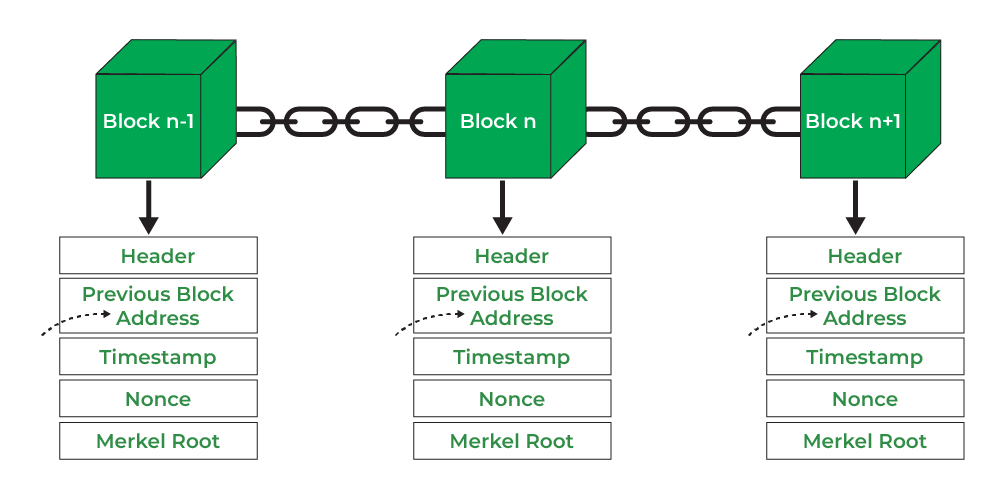
\includegraphics[scale=0.45]{gambar/bab2/Structureofblocksinblockchain.png}
  \caption{Struktur Blockchain \parencite{BlockchainStructure}}
  \label{fig:BlockchainStructure}
\end{figure}

Salah satu aspek penting dari blockchain adalah skalabilitasnya. Saat ini,
skalabilitas dianggap sebagai hambatan utama dalam infrastruktur blockchain.
Blockchain memiliki potensi untuk bersaing dengan jaringan pembayaran
elektronik terbesar, tetapi kemampuannya terbatas pada jumlah transaksi per
detik (TPS) yang dapat ditangani. Sebagai ilustrasi, dua blockchain paling
terkenal saat ini adalah Bitcoin, yang dapat memproses 4,6 TPS, dan Ethereum,
yang mampu menangani sekitar 14,3 TPS (nilai ini sedikit bervariasi). Sebagai
perbandingan, salah satu jaringan pembayaran elektronik terbesar, Visa, dapat
memproses sekitar 1.736 TPS dan bahkan mencapai puncak hingga 47.000 TPS.Saat
ini, blockchain Bitcoin menghasilkan satu blok baru setiap 10 menit (waktu
pembuatan blok atau Time Block generation, TB) dengan ukuran blok (B) sebesar 1
MB (1.048.576 byte). Rata-rata ukuran transaksi adalah 380 byte.

Berbeda dari yang mungkin diperkirakan, masalah skalabilitas tidak dapat
diselesaikan hanya dengan mengubah parameter seperti ukuran blok (B) atau waktu
pembuatan blok (TB). Ada faktor penting yang harus diperhatikan, yaitu waktu
relay (Time Relay, TR), yaitu waktu yang diperlukan untuk menyebarkan blok baru
ke semua node dalam jaringan. TR ini menentukan batas bawah waktu pembuatan
blok (TB), di mana jika TB lebih kecil dari TR, maka node dalam jaringan tidak
akan bisa terus diperbarui. Sebagai contoh, pada blockchain Bitcoin pada
Januari 2021, diperkirakan terdapat sekitar 10.000 node dalam jaringan. Waktu
rata-rata untuk menyebarkan satu blok ke 99\% node dalam jaringan adalah
sekitar 14 detik. Oleh karena itu, TB tidak bisa lebih rendah dari 14 detik,
karena jika blok baru dibuat sebelum blok lama diterima oleh sebagian besar
node, maka jaringan akan mengalami masalah sinkronisasi. Masalah lain muncul
ketika ukuran blok (B) diperbesar. Jika jumlah data yang harus disebarkan ke
jaringan meningkat, waktu relay 14 detik mungkin tidak lagi cukup untuk
memastikan semua node menerima informasi tersebut. Pada tahun 2017, soft fork
Segregated Witness (SegWit) membantu meningkatkan ukuran blok secara efektif
hingga 4 MB (meskipun dalam praktiknya hanya sekitar 2 MB) tanpa mengubah kode
inti blockchain. Namun, peningkatan ini tidak cukup untuk meningkatkan TPS
secara signifikan dan tidak menyelesaikan masalah skalabilitas secara
menyeluruh.

\section{Ethereum dan Layer-2}
\label{sec:ethereumdanlayer2}

Vitalik Buterin adalah pendiri Ethereum, sebuah platform blockchain publik yang
pertama kali diperkenalkan pada tahun 2013 melalui makalah awalnya. Ethereum
bertujuan menyediakan solusi sederhana dan umum bagi pengembang untuk membangun
aplikasi terdesentralisasi berbasis blockchain menggunakan smart contract. Pada
tahun 2016, Buterin menerbitkan makalah tinjauan yang menjelaskan desain dasar
Ethereum secara lebih sederhana. Infrastruktur Ethereum didasarkan pada
blockchain publik yang menggunakan algoritma konsensus bernama
Ethash.\parencite{Buterin2016} Meskipun serupa dengan mekanisme
\emph{proof-of-work} (PoW) pada Bitcoin, Ethash memiliki prinsip kerja yang
berbeda. Proses mining di Bitcoin bergantung pada daya CPU yang secara
terus-menerus menghitung nilai hash kompleks menggunakan algoritma SHA (Secure
Hash Algorithm) (Eastlake \& Jones, 2001) hingga kondisi tertentu terpenuhi.
Hal ini mendorong pengembangan \emph{application-specific integrated circuit}
(ASIC), perangkat keras khusus untuk mining, yang dianggap tidak cocok untuk
Ethereum. Oleh karena itu, Ethash dirancang dengan fungsi hash berbasis memori
\emph{memory-hard hash} untuk mengoptimalkan kinerja memori perangkat, bukan
CPU atau GPU, guna mencegah dominasi ASIC dalam jaringan Ethereum.

Keunggulan utama Ethereum adalah lapisan fungsional abstrak yang berjalan di
atas sebuah jaringan blockchain. Ethereum menggunakan \emph{virtual machine}
bernama \emph{Ethereum Virtual Machine} yang bersifat \emph{Turing-complete},
yang memungkinkan pengembang membangun aplikasi terdesentralisasi tanpa perlu
membuat blockchain baru. EVM menginterpretasikan \emph{smart contract} menjadi
kode yang dapat dijalankan di blockchain Ethereum. Tidak seperti Bitcoin yang
membatasi penggunaan loop untuk mencegah loop tak berujung selama verifikasi
transaksi, Ethereum mendukung loop berkat EVM, menjadikannya
\emph{Turing-complete}. Namun, seiring berkembangnya penggunaan Ethereum,
muncul tantangan skalabilitas yang mendorong pengembangan solusi \emph{Layer
  2}. Pendekatan ini membangun kerangka kerja yang menangani transaksi di luar
rantai utama (\emph{off-chain}), sehingga mengurangi beban pada blockchain
utama dan juga meningkatkan kecepatan transaksi.\emph{Solusi Layer 2} adalah
protokol sekunder yang dibangun di atas blockchain yang sudah ada, di mana
transaksi dilakukan \emph{off-chain} dan hanya `ringkasan' transaksi tersebut
yang dicatat di rantai utama. Ada beberapa jenis solusi Layer 2 yang umum
digunakan, seperti \emph{channels}, \emph{sidechains}, dan \emph{rollups}.
\emph{Channels} menciptakan jalur komunikasi langsung atau tidak langsung
\emph{off-chain} antara node, dengan contoh implementasi seperti \emph{Raiden
  Network} untuk Ethereum. Sementara \emph{sidechains} adalah blockchain `anak'
yang terhubung dengan rantai utama dan berjalan secara paralel, dengan
\emph{Plasma} sebagai contoh arsitektur khususnya.\emph{Rollups} berbeda karena
tetap mencatat data transaksi di rantai utama meskipun eksekusinya dilakukan
\emph{off-chain}.

\emph{The Merge} adalah pembaruan besar dalam ekosistem Ethereum yang terjadi pada September 2022, di mana mekanisme konsensus Ethereum beralih dari \emph{Proof of Work} (PoW) ke \emph{Proof of Stake} (PoS). Sebelum \emph{The Merge}, Ethereum menggunakan algoritma PoW bernama Ethash untuk memvalidasi transaksi dan menambang blok baru, yang membutuhkan energi komputasi tinggi dan perangkat keras khusus. Dengan beralih ke PoS, Ethereum menggantikan proses mining dengan mekanisme di mana validator memilih dan memvalidasi blok berdasarkan jumlah Ether (\emph{stake}) yang mereka pertaruhkan sebagai jaminan. Validator yang bertanggung jawab menjalankan node dan melakukan verifikasi transaksi akan mendapatkan imbalan dalam bentuk Ether, sedangkan validator yang mencoba melakukan kecurangan dapat kehilangan sebagian atau seluruh stake mereka.

\subsection{Zero-Knowledge Rollup (ZK Rollup)}
\label{sec:zkrollup}
Zero-Knowledge Rollup (ZK Rollup) adalah solusi scaling Layer-2 yang
meningkatkan throughput jaringan blockchain dengan memproses banyak transaksi
secara off-chain dan mengirimkan bukti kriptografi ke rantai utama (mainnet).
Teknologi ini menggabungkan keunggulan \emph{zero-knowledge proof} dengan
teknik \emph{rollup} untuk mencapai skalabilitas tinggi sekaligus
mempertahankan keamanan Layer-1. ZK Rollup mengumpulkan ratusan transaksi
off-chain dan mengompilasinya menjadi satu transaksi tunggal dengan
menghasilkan bukti kriptografi yang disebut ZK-SNARK (Zero-Knowledge Succinct
Non-Interactive Argument of Knowledge). Bukti ini memverifikasi bahwa seluruh
transaksi dalam batch valid tanpa perlu memverifikasi masing-masing transaksi
secara individual di mainnet \parencite{Chaliasos2023}. Proses implementasi ZK
Rollup secara umum meliputi beberapa tahapan: pengguna mengirimkan transaksi ke
operator ZK Rollup, operator mengumpulkan transaksi dalam batch, kemudian smart
contract khusus menghasilkan bukti ZK untuk batch tersebut. Bukti dan data
status dikirim ke kontrak di mainnet, yang kemudian memverifikasi bukti dan
memperbarui status blockchain. Beberapa implementasi ZK Rollup yang populer di
industri blockchain termasuk zkSync dari Matter Labs, Polygon zkEVM yang
menghadirkan kompatibilitas penuh dengan Ethereum Virtual Machine (EVM), serta
StarkNet yang menggunakan bahasa pemrograman Cairo untuk smart contract. Setiap
implementasi memiliki karakteristik dan trade-off masing-masing dalam hal
skalabilitas, kompatibilitas, dan kompleksitas yang perlu dipertimbangkan saat
penggunaannya. \parencite{Wackerow2024}

\section{Polygon zkEVM}
\label{sec:polygonzkevm}
\emph{Polygon zkEVM} adalah implementasi \emph{Zero-Knowledge Rollup} yang dirancang khusus untuk memberikan kompatibilitas penuh dengan \emph{Ethereum Virtual Machine (EVM)}. Dengan kata lain, \emph{smart contract} yang sudah ada di \emph{Ethereum} dapat dijalankan secara langsung di \emph{Polygon zkEVM} tanpa perlu penyesuaian kode signifikan. Teknologi \emph{zkEVM} menggunakan bukti kriptografi \emph{zero-knowledge} untuk memverifikasi eksekusi transaksi \emph{off-chain} dan hanya mengirimkan bukti tersebut ke rantai utama \emph{Ethereum}, sehingga mengurangi beban penyimpanan dan perhitungan di \emph{mainnet}. Pendekatan ini memungkinkan \emph{throughput} transaksi yang jauh lebih tinggi dan biaya \emph{gas} yang lebih rendah dibandingkan transaksi langsung di \emph{Ethereum Layer-1} \parencite{polygon2024}. \emph{Polygon zkEVM} juga mempertahankan keamanan dari rantai utama \emph{Ethereum} dengan mengandalkan mekanisme konsensus dan \emph{finalitas} yang sudah teruji, sehingga memberikan solusi skalabilitas yang efektif tanpa mengorbankan desentralisasi atau keamanan. Implementasi ini cocok untuk aplikasi yang membutuhkan performa tinggi dengan biaya rendah, sambil tetap menjaga interoperabilitas penuh dengan ekosistem \emph{Ethereum} yang sudah ada.

\begin{figure} [H] \centering
  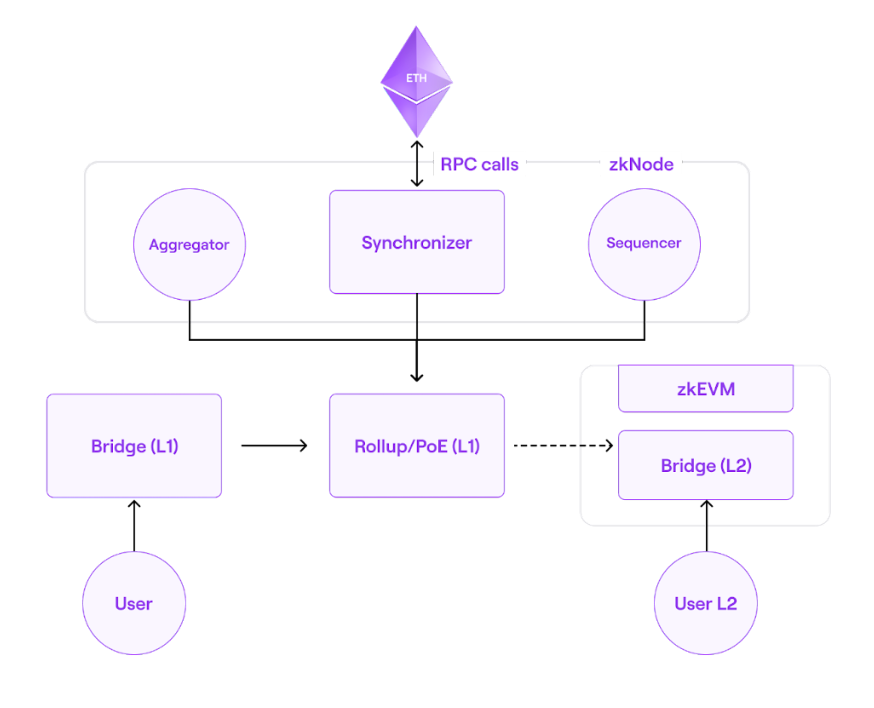
\includegraphics[scale=0.65]{gambar/bab2/zkevm.png}
  \caption{Diagram Polygon zkEVM \parencite{PolygonzkEVMDiagram}}
  \label{fig:PolygonzkEVMDiagram}
\end{figure}

% \begin{figure}[H]
%   \centering

%   % Ubah dengan nama file gambar dan ukuran yang akan digunakan
%   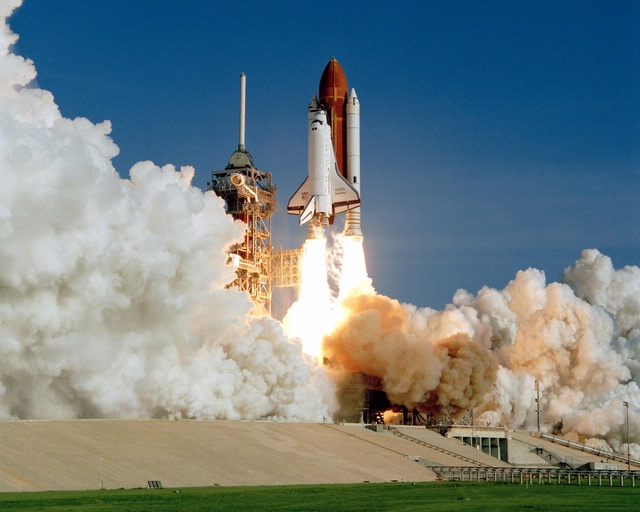
\includegraphics[scale=0.35]{gambar/roketluarangkasa.jpg}

%   % Ubah dengan keterangan gambar yang diinginkan
%   \caption{Peluncuran roket luar angkasa \emph{Discovery} \parencite{roketluarangkasa}.}
%   \label{fig:roketluarangkasa}
% \end{figure}

Gambar \ref{fig:PolygonzkEVMDiagram} merupakan arsitektur sistem
\emph{blockchain} yang tergambar dalam diagram ini menyajikan solusi
komprehensif untuk penskalaan \emph{Ethereum} melalui implementasi
\emph{Layer-2 (L2)} yang terstruktur secara strategis. Pada hierarki teratas,
terdapat jaringan utama \emph{Ethereum (ETH)} yang berfungsi sebagai lapisan
keamanan fundamental dan titik anker kepercayaan bagi seluruh ekosistem.
\emph{Ethereum} terhubung dengan komponen \emph{Synchronizer} melalui panggilan
\emph{Remote Procedure Call (RPC)} yang memungkinkan komunikasi dua arah antara
jaringan utama dan lapisan penskalaan. \emph{Synchronizer} berperan sebagai
jembatan komunikasi krusial yang memastikan konsistensi data dan status antara
\emph{Layer-1} dan \emph{Layer-2}, sambil berkoordinasi dengan
\emph{Aggregator} dan \emph{Sequencer} yang berada dalam infrastruktur
\emph{zkNode}. \emph{Aggregator} bertanggung jawab mengumpulkan dan
menggabungkan transaksi dari berbagai sumber menjadi \emph{batch} teroptimasi,
sementara \emph{Sequencer} mengatur urutan eksekusi transaksi dengan presisi
untuk menjaga konsistensi dan keadilan dalam sistem. sAlur proses transaksi
dimulai ketika \emph{User} berinteraksi dengan \emph{Bridge (L1)}, sebuah
protokol penghubung yang memfasilitasi transfer aset dan informasi dari
\emph{Ethereum} ke sistem \emph{Rollup/PoE (\emph{Proof of Efficiency})} pada
\emph{Layer-1}. \emph{Rollup/PoE} merupakan teknologi inovatif yang
mengumpulkan sejumlah besar transaksi, mengeksekusinya di luar rantai utama,
dan kemudian mengompresi hasil komputasinya menjadi bukti kriptografis yang
ringkas namun terverifikasi. Dari \emph{Rollup}, terbentuk hubungan dengan
\emph{zkEVM} dan \emph{Bridge (L2)} yang ditandai dengan garis putus-putus,
mengindikasikan jalur komunikasi yang bersifat kondisional atau tidak selalu
aktif. \emph{zkEVM (\emph{Zero-Knowledge Ethereum Virtual Machine})} merupakan
implementasi revolusioner dari mesin virtual \emph{Ethereum} yang memanfaatkan
kriptografi \emph{zero-knowledge} untuk memverifikasi komputasi tanpa
mengungkapkan data sensitif, secara dramatis meningkatkan privasi dan efisiensi
pemrosesan. Pada sisi lain, \emph{User L2} dapat langsung berinteraksi dengan
\emph{Bridge (L2)}, memberikan akses yang lebih cepat dan hemat biaya ke
fungsionalitas \emph{blockchain} melalui lapisan penskalaan.

\section{\emph{Non-Fundgible Token (NFT)}}
\label{sec:nft}
Token \emph{non-fungible (NFT)} berbeda dari token fungible dalam dua aspek penting: setiap \emph{NFT} bersifat unik dan tidak dapat dibagi atau digabungkan (Voshmgir, 2018). Bentuk baru token ini pertama kali diperkenalkan melalui standar ERC-721 pada akhir tahun 2017 \parencite{entriken2018}. \emph{ERC-721} memiliki perbedaan signifikan dibandingkan dengan standar \emph{ERC-20} karena memperluas antarmuka umum untuk token dengan fungsi tambahan yang memastikan token berbasis standar ini bersifat non-fungible dan unik \parencite{entriken2018}. Karakteristik khusus ini membuka berbagai peluang baru bagi praktisi. \emph{NFT} memungkinkan tokenisasi aset individu, sesuatu yang sulit dilakukan dengan token fungible karena token tersebut tidak dapat secara digital merepresentasikan keunikan. Oleh karena itu, praktisi telah melakukan berbagai eksperimen menggunakan \emph{NFT} untuk merepresentasikan barang digital seperti aset permainan virtual, karya seni digital, dan lisensi perangkat lunak, serta aset fisik seperti barang mewah dan mobil \parencite{butcher2018}\parencite{griffin2018}. \emph{NFT} juga dipandang sebagai kunci untuk membuka pasar koleksi, yang memiliki estimasi nilai pasar global sebesar USD 200 miliar \parencite{fenech2018}.

Meskipun telah muncul berbagai contoh penggunaan eksperimental, pemahaman yang
lebih mendalam tentang \emph{NFT} akan sangat bermanfaat dari sudut pandang
penelitian Sistem Informasi (IS) dalam tiga aspek utama. Pertama, pengetahuan
deskriptif yang solid tentang karakteristik umum \emph{NFT} dan perbedaannya
dengan token fungible dapat membantu memahami manfaat serta peluang yang
dihasilkan. Kedua, pengetahuan preskriptif yang lebih baik tentang proses
perancangan dan evaluasi aplikasi berbasis \emph{NFT} akan membantu peneliti
dan praktisi. Ketiga, peningkatan kesadaran terhadap tantangan praktis dapat
membantu peneliti di masa depan lebih fokus pada penyelesaian tantangan yang
tersisa. Sayangnya, penelitian mendalam oleh akademisi yang menyentuh
aspek-aspek ini masih sangat terbatas. Selain itu, literatur saat ini
kekurangan praktik terbaik, pengalaman proyek pengembangan, dan wawasan tentang
pengembangan perangkat lunak berbasis blockchain \parencite{delmolino2016}.

\section{Smart Contract}
\label{sec:smartcontract}
\emph{Smart Contract} adalah sekumpulan aturan dan logika prosedural berbasis skenario dan respons. Dengan kata lain, \emph{smart contract} adalah kode terdesentralisasi dan terpercaya yang dijalankan di blockchain. Pihak-pihak yang menandatangani kontrak harus sepakat mengenai detail kontrak, kondisi pelanggaran, tanggung jawab atas pelanggaran, serta sumber data eksternal untuk verifikasi. Setelah kesepakatan tercapai, kontrak ini kemudian diterapkan di blockchain dalam bentuk \emph{smart contract} untuk mengotomatisasi pelaksanaan perjanjian atas nama para penandatangan. Seluruh proses ini berjalan tanpa keterlibatan lembaga pusat apa pun. Mekanisme kerja \emph{smart contract} dapat digambarkan pada gambar 2.3. Biasanya, setelah semua pihak menandatangani \emph{smart contract}, kontrak tersebut dilampirkan ke blockchain dalam bentuk kode program (misalnya, seperti transaksi Bitcoin). Kontrak ini kemudian dicatat dalam blockchain setelah disebarluaskan melalui jaringan \emph{peer-to-peer} (P2P) dan diverifikasi oleh node.\emph{smart contract} mencakup sejumlah status yang telah ditentukan sebelumnya, aturan transisi, skenario yang memicu eksekusi kontrak (seperti waktu tertentu atau terjadinya suatu peristiwa), serta respons terhadap skenario tersebut. Blockchain memantau status real-time dari \emph{smart contract} dan mengeksekusinya ketika kondisi pemicu tertentu telah terpenuhi\parencite{delmolino2016}.

\begin{figure} [H] \centering
  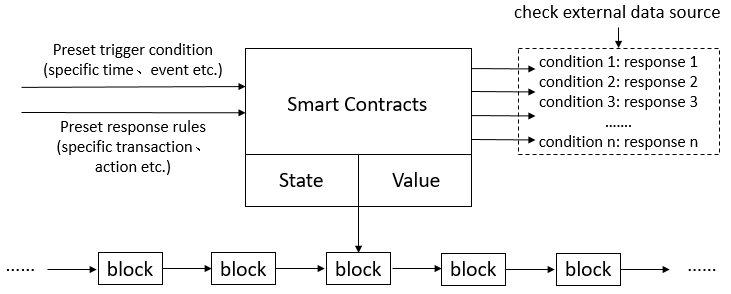
\includegraphics[scale=0.45]{gambar/bab2/The-mechanism-of-smart-contracts.png}
  \caption{Mekanisme \emph{Smart Contract} \parencite{SmartContractStructure}}
  \label{fig:SmartContractStructure}
\end{figure}

\section{IPFS}
\label{sec:ipfs}
IPFS (InterPlanetary File System) adalah protokol peer-to-peer yang dirancang
agar memungkinkan pengguna berbagi data melalui sistem file terdistribusi.
Mirip dengan blockchain, IPFS mengandalkan jaringan node-node yang saling
terhubung untuk menyimpan data. Sistem ini menggunakan Distributed Hash Table
(DHT) sebagai mekanisme untuk menemukan lokasi data dengan efisien. Ketika file
diunggah ke IPFS, file tersebut dipecah menjadi beberapa bagian kecil yang
disebut chunk, di mana setiap chunk saling terhubung melalui tautan unik.
Struktur ini memungkinkan data untuk diakses dengan cepat dan efisien di
seluruh jaringan.Salah satu fitur unggulan IPFS adalah adanya fungsi
versioning, yang memungkinkan pengguna untuk memperbarui file yang telah
diunggah dan mencatat seluruh perubahan yang terjadi. Dengan adanya fitur ini,
pengguna tidak hanya dapat melacak riwayat perubahan, tetapi juga memastikan
integritas data. Teknologi ini cocok digunakan dalam berbagai aplikasi yang
membutuhkan pengelolaan file secara terdistribusi, seperti penyimpanan file
yang aman, berbagi konten, atau mendukung infrastruktur web yang
terdesentralisasi. IPFS juga menjadi solusi untuk mengurangi ketergantungan
pada server terpusat, menjadikannya lebih tahan terhadap kegagalan jaringan dan
serangan siber \parencite{steichen2018}.

\section{ Penelitian Terdahulu}
\label{sec:penelitianterdahulu}

Beberapa penelitian terdahulu telah membahas implementasi blockchain dan NFT
dalam sistem manajemen tiket acara, yang menjadi dasar penting bagi
pengembangan sistem tiket berbasis NFT yang lebih canggih dan efisien. Salah
satu pendekatan yang dikembangkan adalah sistem tiket berbasis blockchain
hybrid yang menggabungkan kelebihan blockchain publik dan private. Penelitian
ini mengusulkan arsitektur yang menggunakan blockchain private untuk manajemen
tiket internal, serta blockchain publik untuk verifikasi tiket. Keunggulan
utama pendekatan hybrid ini meliputi peningkatan skalabilitas dengan mengurangi
beban pada blockchain publik, penurunan biaya operasional melalui pemindahan
sebagian transaksi ke blockchain private, dan pemeliharaan transparansi serta
keamanan melalui integrasi dengan blockchain publik. Namun, implementasi sistem
hybrid ini memerlukan infrastruktur yang lebih kompleks serta koordinasi yang
baik antara kedua jenis blockchain.

Kontribusi signifikan lainnya berasal dari penelitian \parencite{Regner2019}.\
yang melakukan studi komprehensif mengenai penggunaan NFT dalam aplikasi tiket
berbasis blockchain. Penelitian tersebut mengembangkan prototipe sistem tiket
berbasis NFT di platform Ethereum dan menganalisis efektivitas smart contract
dalam mencegah scalping tiket. Studi ini juga mengevaluasi dampak ekonomis
implementasi NFT dalam industri tiket, menunjukkan bahwa NFT dapat secara
efektif mengatasi pemalsuan tiket dan penjualan kembali yang tidak terkendali,
walaupun tantangan terkait biaya gas pada jaringan Ethereum masih ada.
Penelitian oleh Srinivasarao et al.\ lebih berfokus pada aspek praktis
implementasi blockchain dalam manajemen tiket acara. Mereka mengembangkan
sistem manajemen tiket terdesentralisasi, mekanisme verifikasi tiket berbasis
blockchain, serta melakukan analisis performa dan skalabilitas sistem.
Penelitian ini memberikan wawasan berharga mengenai tantangan teknis, terutama
terkait skalabilitas dan kinerja sistem tiket berbasis blockchain.

Berdasarkan tinjauan terhadap penelitian-penelitian terdahulu, dapat
diidentifikasi beberapa gap yang akan diisi oleh penelitian ini. Implementasi
solusi Layer 2 Ethereum untuk mengatasi masalah skalabilitas dan biaya
transaksi masih kurang dieksplorasi secara mendalam. Penelitian ini bertujuan
untuk mengisi gap-gap tersebut dengan mengembangkan sistem tiket berbasis NFT
yang terintegrasi dengan Web 3.0, mengimplementasikan solusi Layer 2 seperti
Polygon zkEVM, serta memberikan analisis mendalam terkait dampak implementasi
dalam konteks industri musik di Indonesia.

% % Contoh input gambar
% \begin{figure}[H]
%   \centering

%   % Ubah dengan nama file gambar dan ukuran yang akan digunakan
%   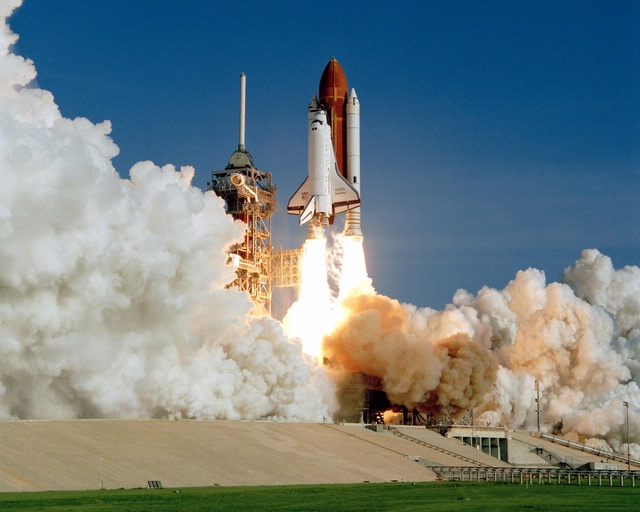
\includegraphics[scale=0.35]{gambar/roketluarangkasa.jpg}

%   % Ubah dengan keterangan gambar yang diinginkan
%   \caption{Peluncuran roket luar angkasa \emph{Discovery} \parencite{roketluarangkasa}.}
%   \label{fig:roketluarangkasa}
% \end{figure}

% Roket luar angkasa merupakan \lipsum[1]

% \emph{Discovery}, Gambar \ref{fig:roketluarangkasa}, merupakan \lipsum[2]

% \section{Gravitasi}
% \label{sec:gravitasi}

% Gravitasi merupakan \lipsum[1]

% \subsection{Hukum Newton}
% \label{subsec:hukumnewton}

% Newton \parencite{newton1687} pernah merumuskan bahwa \lipsum[1] Kemudian
% menjadi persamaan seperti pada persamaan \ref{eq:hukumpertamanewton}.

% % Contoh pembuatan persamaan
% \begin{equation}
%   \label{eq:hukumpertamanewton}
%   \sum \mathbf{F} = 0\; \Leftrightarrow\; \frac{\mathrm{d} \mathbf{v} }{\mathrm{d}t} = 0.
% \end{equation}

% \subsection{Anti Gravitasi}
% \label{subsec:antigravitasi}

% Anti gravitasi merupakan \lipsum[1]
